\documentclass[11pt]{article}
\usepackage[norsk]{babel}
\usepackage[utf8]{inputenc}
\usepackage{hyperref}
\usepackage{amsmath}
\usepackage{amssymb}
\usepackage{amsthm}
\usepackage{wasysym}
\usepackage{sectsty}
%\usepackage{fullpage}
\usepackage{graphicx}

% Disse kommandoene definerer hvor stor andel av siden som kan være dekket av figurer. Kan gjøre det enklere å plassere figurer.
\setcounter{totalnumber}{15}
\renewcommand{\textfraction}{0.05}
\renewcommand{\topfraction}{0.95}
\renewcommand{\bottomfraction}{0.95}
\renewcommand{\floatpagefraction}{0.35}


\newcommand\numberthis{\addtocounter{equation}{1}\tag{\theequation}}
\renewcommand{\thesection}{}
\renewcommand{\thesubsection}{}

\usepackage{fancyhdr} % Custom headers and footers
\pagestyle{fancyplain} % Makes all pages in the document conform to the custom headers and footers
\fancyhead[C]{\footnotesize \textit{FYS3150 Prosjekt 1\\ $ \,$}} % header
\fancyhead[R]{} \fancyhead[L]{} \fancyfoot[L]{} % Empty left footer
\fancyfoot[C]{} % Empty center footer
\fancyfoot[R]{\thepage} % Page numbering for right footer
\renewcommand{\headrulewidth}{0pt} % Remove header underlines
\renewcommand{\footrulewidth}{0pt} % Remove footer underlines
\setlength{\headheight}{21pt} % Customize the height of the header

\newcommand{\horline}{
\begin{center}
\line(1,0){350}
\end{center}
}

% common commands
\newcommand{\pd}[2] {\frac{\partial #1}{\partial #2}}
\renewcommand{\div}[1] {\nabla\cdot\vec{#1}}
\newcommand{\curl}[1] {\nabla\times\vec{#1}}
\renewcommand{\vec}{\mathbf} % bold face for vectors
\newcommand{\e}[1] {\times 10^{#1}}
\newcommand{\mean}[1] {\langle #1 \rangle}

\begin{document}
% make title page
\begin{titlepage}
\newcommand{\HRule}{\rule{\linewidth}{0.5mm}}
\center
\textsc{\LARGE Universitetet i Oslo}\\[1.5cm] % Name of your university/college
\textsc{\Large }\\[0.5cm] % Major heading such as course name
\textsc{\large FYS3150}\\[0.5cm] % Minor heading such as course title
\HRule \\[0.4cm]
{ \huge \bfseries Prosjekt 1 }\\[0.4cm] % Title of your document
\HRule \\[1.5cm]
\Large \emph{Skrevet av:}\\
Lyder \textsc{Rumohr Blingsmo} og Bendik \textsc{Samseth}\\[3cm]
{\large \today}\\[3cm]
\vfill
\end{titlepage}


\begin{abstract}
I dette prosjektet skal vi kjent med ulike vektor- og
matriseoperasjoner. Vi skal benytte C++ for størsteparten av
beregningene i et forsøk på å bli bedre kjent med språket. Vi ser på
andreordens lineære differensialligninger, spesielt ser vi på den
generelle endimensjonelle Poisson ligningen med Dirichlet
randbetingelser. Vi ser på flere måter å løse slike systemer, og
analyserer forskjellene med tanke på kjøretid og nøyaktighet. All
programkode brukt til å finne resultatene presentert her er
tilgjengelig på
\href{https://github.com/bsamseth/fys3150-project1}{GitHub}\footnote{\label{GitHub-link}Dersom
  linken ikke er tilgjenngelig er eksplisitt adresse: \url{https://github.com/bsamseth/fys3150-project1}}
\end{abstract}


Vi har gitt den generelle formen til den endimensjonelle
Possionsligningen:
\begin{align}
  -u''(x) = f(x)\label{eq:poisson}
\end{align}
med $x \in (0,1)$ og $u(0) = u(1) = 0$.

\subsection{Diskretisering av problemet}

For å komme frem til en numerisk løsning til \eqref{eq:poisson}
definerer vi den diskretiserte tilnærmingen til $u(x)$ som $v_i$ med
x-verdier $x_i = ih$ på intervallet $x_0 = 0$ og $x_{n+1} =
1$. Avstanden mellom hver $x_i$ defineres som $h =
1/(n+1)$. Randbetingelsene blir da $v_0 = v_{n+1} = 0$.

Ligning \eqref{eq:poisson} viser at vi trenger den dobbeltderiverte av
$u(x)$. For $v_i$ kan vi tilnærme dette som 

\begin{align}
  - \frac{ v_{i+1} + v_{i-1} - 2v_i }{ h^2 } =
  f_i\hspace{1cm}\text{for } i = 1,\dots,n.
\end{align}
der $f_i = f(x_i)$. Vi setter 
\begin{align*}
      {\bf A} = \left(\begin{array}{cccccc}
                           2& -1& 0 &\dots   & \dots &0 \\
                           -1 & 2 & -1 &0 &\dots &\dots \\
                           0&-1 &2 & -1 & 0 & \dots \\
                           & \dots   & \dots &\dots   &\dots & \dots \\
                           0&\dots   &  &-1 &2& -1 \\
                           0&\dots    &  & 0  &-1 & 2 \\
                      \end{array} \right)
\end{align*}
Da ser vi at $\vec A \vec v$ blir lik 
\begin{align*}
  \vec A \vec v = -v_{i+1} - v_{i-1} + 2v_i\hspace{1cm}\text{for } i = 1,\dots,n
\end{align*}
når vi har at $v_0 = v_{n+1} = 0$ fra Dirichlet-randbetingelsene. Hvis
vi definerer $\vec d$ ved $d_i = h^2f_i$ kan vi skrive
\eqref{eq:poisson} som 
\begin{align}
  \vec A \vec v = \vec d.\label{Av=d}
\end{align}
 

Vi skal videre anta at $f(x) = 100 e^{-10x}$. Da har
\eqref{eq:poisson} en eksakt løsning gitt som
 \begin{align}
u(x) = 1 -\left(1-e^{-10}\right) - e^{-10x}.\label{eq:exact}
\end{align} 
Vi skal bruke denne til å
sammenlikne med vår numeriske lønning i senere oppgaver.

\subsection{Metode for løsning}
For å løse \eqref{Av=d} skal vi benytte en noe modifisert version av
Thomas algoritmen\footnote{Se
  \url{https://en.wikipedia.org/wiki/Tridiagonal_matrix_algorithm}}. Denne
algoritmen kan beskrives som følger: 

Gitt 
\begin{align*}
  \begin{bmatrix}
   {b_1} & {c_1} &  &  & \text{\huge0} \\
   {a_2} & {b_2} & {c_2} &  &  \\
    & {a_3} & {b_3} & \ddots &  \\
    &  & \ddots & \ddots & {c_{n-1}}\\
     \text{\huge0}&  &  & {a_n} & {b_n}\\
\end{bmatrix}
\begin{bmatrix}
   {x_1 }  \\
   {x_2 }  \\
   {x_3 }  \\
   \vdots   \\
   {x_n }  \\
\end{bmatrix}
=
\begin{bmatrix}
   {d_1 }  \\
   {d_2 }  \\
   {d_3 }  \\
   \vdots   \\
   {d_n }  \\
\end{bmatrix}.
\end{align*}
Vi kan løse systemet ved å utføre en forward-substitution bestående av
å bytte ut matrise elementene $c_i$ og $d_i$ med $c_i'$ og $d_i'$ på følgende måte.
\begin{align*}
  c_i' &= \begin{cases}
\begin{array}{lcl}
  \cfrac{c_i}{b_i}                  & ; & i = 1 \\
  \cfrac{c_i}{b_i - a_i c'_{i - 1}} & ; & i = 2, 3, \dots, n-1 \\
\end{array}
\end{cases}\\
d_i' &= \begin{cases}
\begin{array}{lcl}
  \cfrac{d_i}{b_i}                  & ; & i = 1 \\
  \cfrac{d_i - a_i d'_{i - 1}}{b_i - a_i c'_{i - 1}} & ; & i = 2, 3, \dots, n. \\
\end{array}
\end{cases}
\end{align*}
Deretter finner vi løsningen ved backward-substitution.
\begin{align*}
  x_n &= d'_n\\
  x_i &= d'_i - c'_i x_{i + 1} \qquad ; \ i = n - 1, n - 2, \ldots, 1.
\end{align*}

Dette teller vi til å tilsvare $\mathcal{O}(10n)$ FLOPS. Siden vi i
vårt tilfellet har like elementer på diagonalene, kan vi trimme dette
ned litt. 

Siden $a_i = -1\ \forall\  i$ og  $b_i - a_ic_{i-1}'$ er fellesnevner
for både $c_i'$ og $d_i'$ kan vi gjøre om forward-substitution til det følgende:

\begin{align*}
  c_i' &= \begin{cases}
\begin{array}{lcl}
  \cfrac{c}{b}                  & ; & i = 1 \\
  \cfrac{c}{b + c'_{i - 1}} & ; & i = 2, 3, \dots, n-1 \\
\end{array}
\end{cases}\\
d_i' &= \begin{cases}
\begin{array}{lcl}
  \cfrac{d_i}{b}                  & ; & i = 1 \\
  \cfrac{d_i + d'_{i - 1}}{b + c'_{i - 1}} & ; & i = 2, 3, \dots, n. \\
\end{array}
\end{cases}
\end{align*}
Her kan vi spare operasjoner ved å bare beregne $b+c'_{i-1}$ en gang
(for alle $i$) og bruke resultatet både for beregningen av $c_{i}'$ og
$d_{i}'$.

Et viktig poeng her er at vi kun bruker algoritmen på de indre
punktene. Vi har Dirichlet-grensebetingelser, så vi skal bare fiksere
$v_1 = v_n = 0$.

Med disse endringene teller vi antall operasjoner til å gå som
$\mathcal{O}(6n)$. Dette er en betydelig raskere algoritme sammenliket
med standard Gauss eliminasjon. I følge forelesningsnotatene går
vanlig Gauss eliminasjon som $\mathcal{O}(\frac{ 2 }{ 3 }n^3)$. I tillegg krever ikke algoritmen vi bruker at vi lagrer en full
matrise. Tridiagonale matriser med stor $n$ inneholder veldig mange
nuller, så det er smart å ikke trenge å lagre all den unødvendige
informasjonen. Dette gjør oss i stand til å løse matriser av mye
større dimensjon sammenliknet med når vi er nødt til å lagre den fulle matrisen.

Vi har implementert dette i C++ ved bruk av standard biblioteket. Full
kildekode finnes i filen \texttt{main.cpp} som er tilgjenngelig på
Github-repoet vårt\footnotemark[1]:

Figur \ref{fig:b} viser resultatet av å bruke denne algoritmen med
$N = \{10,100,1000\}$. Vi ser at $v_i$ konvergerer raskt mot $u(x)$
når vi øker verdien av N. For $N=100$ og $N=1000$ er det vanskelig å
skille den eksakte fra tilnærmingen. Det virker med dette som
algoritmen vi har skrevet fungerer som ønsket.

\begin{figure}[ht]
  \centering
  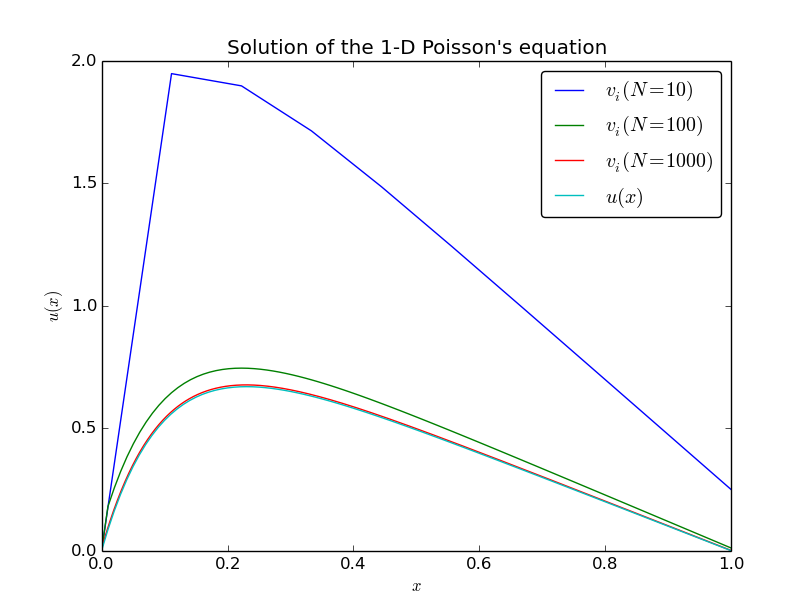
\includegraphics[scale=0.7]{fig/b.png}
  \caption{\label{fig:b} Løsninger av \eqref{eq:poisson} for
    forskjelige verider av N. $u(x)$ viser kurven til den eksakte løsningen.}
\end{figure}

\subsection{Feilanalyse}
Det kan likevel være interessant å se litt mer kvantitativt på hvor
god tilnærmingen vår er. For å gjøre dette har vi skrevet ett program,
\texttt{errorEstimation.py}, som lager et plot av den maksimale
relative differansen mellom $u(x)$ og $v_i$ som funksjon av
steglengden $h = \frac{ 1 }{ n-1 }$. Grafen er vist i figur
\ref{fig:c}. Vi ser en raskt avtagende feil mellom $10^{-1}$ og ned
til $10^{-4}$. Der ser det derimot ut som om vi ikke får mer presisjon
ved å øke verdien av $n$ ytterligere. Vi har latt $n$ gå helt til
$n=10^7$, og ser at presisjonen faktisk minker noe når vi øker $n$
forbi $10^4$. Dette er typisk for denne typen beregninger og kommer av
at vi på et tidspunkt får problemer med presisjonen av hvordan vi
representerer tallene på datamaskinen. Dessuten tar det mye mer tid,
så det virker mye smartere å velge en mer passende verdi for $n$. 

Resultatet er at vi med nokså billig minne- og tidsbruk kan oppnå en
approksimert løsning som har på det minste 5 desimalers
nøyaktighet. 

\begin{figure}[ht]
  \centering
  \includegraphics[scale=0.7]{fig/c.png}
  \caption{\label{fig:c} Maksimal relativ feil mellom eksakt-
    og numerisk approksimert løsning som funksjon av steglengden $h =
    \frac{ 1 }{ n-1 }$. Begge akser er logaritmiske.}
\end{figure}


\subsection{Kjøretid sett i forhold til standardfunksjoner}
Vi ønsker nå å se hvordan vår spesialalgoritme fungerer sammenliknet
med standardfunksjoner tilgjengelig for bruk i C++. Vi har (av
praktiske årsaker) valgt å sammenlikne med Armadillo, der vi benytter
LU-dekomposisjon for å løse \eqref{Av=d}. 

Til dette har vi skrevet et program, \texttt{d.cpp}, som beregner
løsningen først ved hjelp av vår algoritme og deretter ved hjelp av
Armadillo. Vi registrerer tiden det tar fra vi kaller løser-metodene
til vi har fått en ferdig løsning. Vi har altså valgt å ikke inkludere
tiden det tar å sette opp variablene som fôres inn til metodene. 

Før vi går videre må vi bemerke at det er et viktig poeng å komme med
i forhold til allokering av variable. Siden matrisen $A$ er
tridiagonal inneholder den mange nuller, særlig for store $n$. Vår
algoritme krever ikke at vi lagrer mer enn diagonalene og løsningen,
begge som kolonnevektorer. Armadillos funksjoner krever derimot at vi
lagrer den fulle matrisen. Dette gjør at vi må lagre $n\times n$ tall
i matrisen $A$. Hvis vi kjører standardfunksjonene med $n=10^5$ ender
vi opp med en matrise som må lagre $10^{10}$ tall. Dette er mer enn
hva de fleste datamaskiner har mulighet til å lagre i arbeidsminnet,
noe som fører til at vi ikke kan kjøre programmet. Dette setter en
betydelig begrensning på hvor mange punkter vi kan benytte, og dermed
ofte hvor nøyaktig vi kan beregne resultatet.

Vi har valgt å se på kjøretid for $N = \{10, 100, 1000\}$. Resultatet
er gitt i tabell \ref{tab:1}.
\begin{table}[h]
\centering
\caption{Kjøretid for forskjellige verdier av $n$}
\label{tab:1}
\vspace{0.1cm}
\begin{tabular}{rll}
n & Thomas & Armadillo \\
\hline
10 & \input{data/time_data_N_tridiag_10.dat} & \input{data/time_data_N_armaLU_10.dat} \\
100 & \input{data/time_data_N_tridiag_1000.dat} & \input{data/time_data_N_armaLU_100.dat} \\
1000 & \input{data/time_data_N_tridiag_1000.dat} & \input{data/time_data_N_armaLU_1000.dat} \\
\end{tabular}
\end{table}

Vi ser at kjøretiden er dramatisk større når vi bruker Armadillo. Det
er ikke overraskende da vi vet at LU-dekomposisjon bruker noe rundt
$\mathcal{O}(n^3)$ FLOPS, og i tillegg må vi til slutt også løse selve
matriselikningen. Dette gjør at det raskt tar mer tid hvis matrisene
blir større.


\subsection{Konklusjoner}
??? 

\end{document}
%%% Local Variables: 
%%% mode: latex
%%% TeX-master: t
%%% End: 


















